\documentclass{article}
\usepackage[a4paper, margin=1in]{geometry}
\usepackage[T1]{fontenc}
\usepackage[utf8x]{inputenc}
\usepackage{ucs}
\usepackage{xhfill}
\usepackage[spanish]{babel}
\usepackage{url}
\usepackage{tikz}
\usepackage{fancyhdr}
%\usepackage[landscape]{geometry}
\usepackage{amsmath,amsthm,amssymb}
\usepackage{mathrsfs}
\usepackage{dsfont}
\usepackage{upgreek}
\usepackage{graphicx}
\usepackage{svg}
\usepackage{listings}
\usepackage{rotating} 
\usepackage{color} 
\usepackage{wasysym}
\usepackage{hyperref}
\usepackage{multicol}

\definecolor{codegreen}{rgb}{0.08, 0.65, 0.24} 
\definecolor{codewine}{rgb}{0.5, 0.0, 0.5}
\definecolor{codegray}{rgb}{0.63, 0.63, 0.63}
\definecolor{codeblue}{rgb}{0.15, 0.31, 0.78}
\definecolor{backcolour}{rgb}{0.97, 0.97, 0.97}

\lstdefinestyle{villalpando}{
  backgroundcolor=\color{backcolour},   
  commentstyle=\color{codewine},
  keywordstyle=\color{codegreen},
  numberstyle=\tiny\color{codegray},
  stringstyle=\color{codeblue},
  basicstyle=\footnotesize,
  breakatwhitespace=false,         
  breaklines=true,                 
  keepspaces=true,                 
  numbers=left,                    
  numbersep=5pt,                  
  showspaces=false,                
  showstringspaces=false,
  showtabs=false,                  
  tabsize=2
} 
\lstset{style=villalpando}

\pagestyle{fancy}
\fancyhf{}
\renewcommand{\headrulewidth}{0pt}
\lhead{}
\chead{}
\rhead{}
\lfoot{}
\cfoot{\itshape diego.a.villalpando@ciencias.unam.mx}
\rfoot{\thepage}

\begin{document}

%===========Título===========%

{\centering 
\noindent\hrulefill \par \vspace{0.5cm}
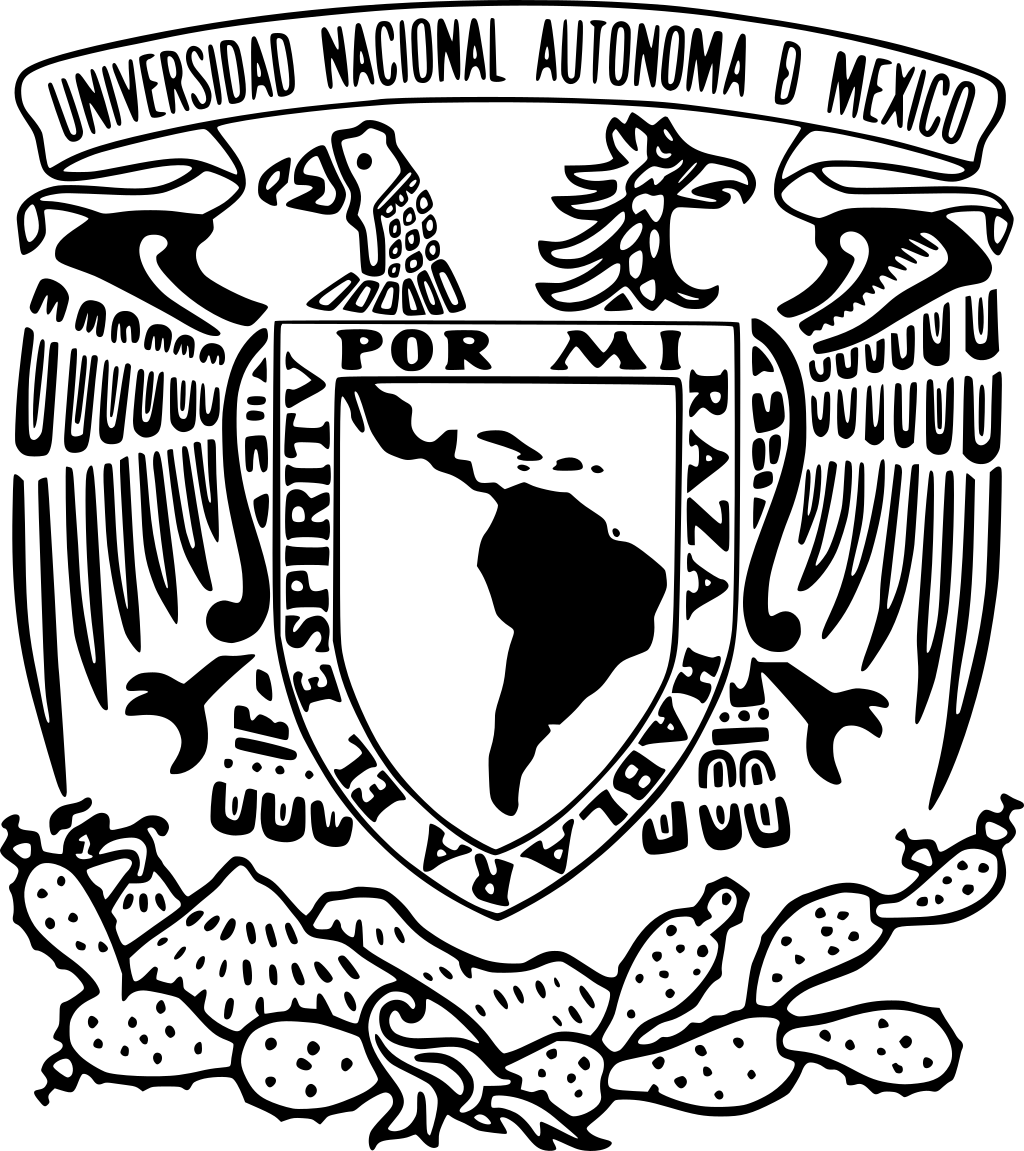
\includegraphics[width=2cm]{unam.png} \hspace{11.5cm}
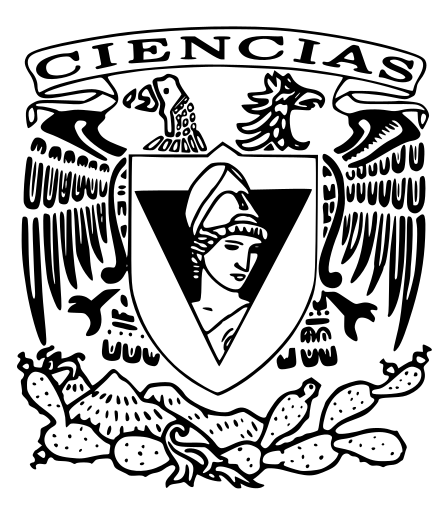
\includegraphics[width=2cm]{ciencias.png}\vspace{-2.2cm}
     {\scshape\Large Universidad Nacional Autónoma de México \par}
     {\scshape\Large Facultad de Ciencias, Ciudad Universitaria \par}
     {\Large Fundamentos de Bases de Datos 7063\par}
     \vspace{0.2cm}
     {\Large\bfseries Normalización de Base de Datos Transpórtate \par}
     \vspace{0.2cm}
     {\large\itshape Diego Alfredo Villalpando Velázquez \par \vspace{0.2cm}}
     {\large\itshape 13 de diciembre de 2019\par} \vspace{0.35cm}
     \noindent\hrulefill
}

%===========Objetivo===========%
\vspace{0.5cm}
       { \bfseries
         Objetivo:
         Se describe a continuación el proceso de normalización a tercera forma normal
         de la base de datos con estructura descrita anteriormente en el pdf anexo
         "disenio.pdf" sobre la empresa ficticia Transpórtate.
       }
       
       % Índice de contenido
       \noindent \tableofcontents

       %===========Introducción===========%
       
       \section{Introducción}
       {
         La empresa Transportate es una empresa de transporte particular con 150 automóviles
         propios para transporte de usuarios ajenos a la empresa y de forma individual. La
         empresa desea crear una base de datos que permita realizar estadísticas
         de los viajes e implementar un nuevo sistema de recompensas para sus clientes
         frecuentes. Se enumeran las reglas de negocio a continuación:
       }
       
       %===========Diseño E/R===========%
       \section{Nuevo Modelo Normalizado en 3NF}

       \subsection{Diagrama Relacional}
       
       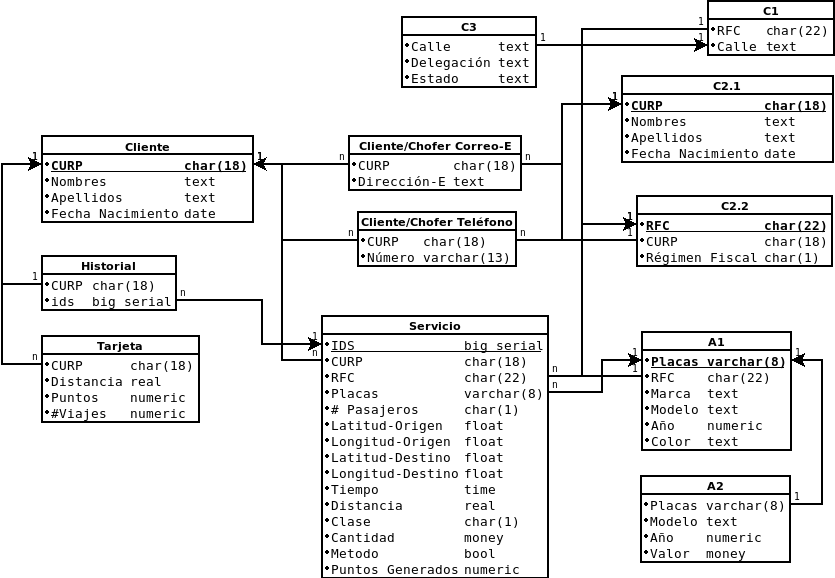
\includegraphics[width=15cm]{RN.png}\\
       \centerline{Diagrama 1: Modelo Relacional normalizado del caso.}\\

       \subsection{Justificación}

       \subsection{Procedimiento}

       \subsubsection{Chofer}
       
       \noindent Con las dependencias funcionales:
       \begin{itemize}
       \item RFC $\rightarrow$ ( CURP, Régimen Fiscal )
       \item CURP $\rightarrow$ ( Nombres, Apellidos, Fecha Nacimiento )
       \item Calle $\rightarrow$ ( Delegación, Estado )
       \end{itemize}\\
       
       \noindent No se encuentra en 3NF, procedemos a normalizar:
       \begin{enumerate}
       \item El alcance mínimo de los atributos en dependencias funcionales son:
         \begin{multicols}{2}
           \begin{itemize}
           \item RFC $\rightarrow$ Régimen Fiscal
           \item RFC $\rightarrow$ CURP
           \item CURP $\rightarrow$ Nombres
           \item CURP $\rightarrow$ Apellidos
           \item CURP $\rightarrow$ Fecha de Nacimiento
           \item Calle $\rightarrow$ Delegación
           \item Calle $\rightarrow$ Estado
           \end{itemize}
         \end{multicols}
       \item Observemos que tenemos dos conjuntos disjuntos de atributos en la relación,
         sus alcances máximos son:
         \begin{itemize}
         \item RFC $\rightarrow$ ( Régimen Fiscal, CURP $\rightarrow$
           ( Nombres, Apellidos, Fecha de Nacimiento ) )
         \item Calle $\rightarrow$ ( Delegación, Estado )
         \end{itemize}
         \end{enumerate}
         Por lo tanto, sus llaves candidatas son RFC y Calle.
       \item Normalizamos a 2NF:
         \begin{enumerate}
         \item Creamos una tabla (C1) con atributos RFC y Calle, las cuales son el 'puente'
           no existente en la tabla original; sin dependencias funcionales.
         \item Creamos las 2 tablas pertenecientes a ambos conjuntos disjuntos de la tabla original:
           \begin{itemize}
           \item (C2) Atributos: RFC, CURP, Régimen Fiscal, Nombres, Apellidos, Fecha Nacimiento.
             Dependencias Funcionales: RFC $\rightarrow$ ( CURP, Régimen Fiscal ) y
             CURP $\rightarrow$ ( Nombres, Apellidos, Fecha de Nacimiento )
           \item (C3) Atributos: Calle, Delegación, Estado. Dependencias Funcionales:
             Calle $\rightarrow$ ( Delegación, Estado )
           \end{itemize}
         \item Eliminamos la tabla original.
         \end{enumerate}
       \item Observemos que las tablas C1 y C3 ya se encuentran en 3NF, pero la tabla C2 no porque
         no tiene una superllave, entonces procedemos a normalizar C2 a 3NF:
         \begin{enumerate}
         \item Creamos la tabla C2.1 con atributos CURP, Nombres, Apellidos, Fecha de Nacimiento.
           Dependencias Funcionales: CURP $\rightarrow$ ( Nombres, Apellidos, Fecha de Nacimiento )
         \item Creamos la tabla C2.2 con atributos RFC, Régimen Fiscal, CURP. Dependencias
           Funcionales: RFC $\rightarrow$ ( Régimen Fidcal, CURP )
         \item Eliminamos la tabla C2.
         \end{enumerate}
       \end{enumerate}
       Hemos terminado de normalizar Choferes a 3NF, creando las tablas C1, C2.1, C2.2, y C3
       en su lugar.
       
      \subsubsection{Automóvil}

      \noindent Con las dependencias funcionales:
      \begin{multicols}{2}
      \begin{itemize}
      \item Placas $\rightarrow$ (RFC, Modelo, Marca, Año, Color)
      \item ( Placas, Modelo, Año ) $\rightarrow$ Valor
      \end{itemize}
      \end{multicols}\\
      
      \noindent No se encuentra en 3NF, procedemos a normalizar:
      \begin{enumerate}
      \item El alcance mínimo de los atributos en dependencias funcionales son:
        \begin{multicols}{2}
          \begin{itemize}
          \item Placas $\rightarrow$ Modelo
          \item Placas $\rightarrow$ Año
          \item Placas $\rightarrow$ Color
          \item Placas $\rightarrow$ Marca
          \item Placas $\rightarrow$ RFC
          \item Modelo Año $\rightarrow$ Valor
          \end{itemize}
        \end{multicols}
      \item Observemos que tenemos un conjunto de atributos relacionados,
        su alcance máximo es:\\
        
        Placas $\rightarrow$ ( Marca, Color, RFC, ( ( Modelo, Año ) $\rightarrow$  Valor ) )

      \item Observemos que Automóviles se encuentra en 2NF, pero viola 3NF por no tener superllave.
        
      \item Normalizamos a 3NF:
        \begin{enumerate}
        \item Creamos una tabla (A1) con atributos Placas, RFC, Modelo, Marca, Año, Color.
          Con dependencia funcional: Placas $\rightarrow$ ( RFC, Año, Modelo, Marca, Color )
        \item Creamos otra tabla (A2) con atributos Modelo, Año, Valor. Con dependencia funcional:\\
          ( Placas, Modelo, Año ) $\rightarrow$ Valor
        \item Eliminamos la tabla original.
        \end{enumerate}
      \item Observemos que las tablas A1 y A2 ya se encuentran en 3NF
      \end{enumerate}
      Hemos terminado de normalizar Automóviles a 3NF, creando las tablas A1 y A2
      en su lugar.
      
      \subsubsection{Servicio}

      \noindent Con las dependencias funcionales:
       \begin{itemize}
       \item IDS $\rightarrow$ CURP, RFC, Placas, $\#$Pasajeros, Clase, Método,
         Latitud Origen, Latitud Destino, Longitud Origen, Longitud Destino, Tiempo, Distancia )
       \item ( Distancia, Tiempo, Clase ) $\rightarrow$ ( Cantidad, Puntos Generados )
       \end{itemize}\\
       
       \noindent No se encuentra en 3NF, procedemos a normalizar:
       \begin{enumerate}
       \item El alcance mínimo de los atributos en dependencias funcionales son:
         \begin{multicols}{2}
           \begin{itemize}
           \item IDS $\rightarrow$ CURP
           \item IDS $\rightarrow$ RFC
           \item IDS $\rightarrow$ Placas
           \item IDS $\rightarrow$ $\#$Pasajeros
           \item IDS $\rightarrow$ Clase
           \item IDS $\rightarrow$ Método
           \item IDS $\rightarrow$ Latitud Origen
           \item IDS $\rightarrow$ Latitud Destino
           \item IDS $\rightarrow$ Longitud Origen
           \item IDS $\rightarrow$ Longitud Destino
           \item IDS $\rightarrow$ Tiempo
           \item IDS $\rightarrow$ Distancia
           \item Distancia Tiempo Clase $\rightarrow$ Cantidad
           \item Distancia Tiempo Clase $\rightarrow$ Puntos Generados
           \end{itemize}
         \end{multicols}
       \item Observemos que tenemos un conjunto relacionado de atributos,
         su alcance máximo es:\\

         IDS $\rightarrow$ ( CURP, RFC, Placas, $\#$Pasajeros, Método, Latitud Origen,
           Latitud Destino, Longitud Origen, Longitud Destino, ( ( Distancia, Tiempo,
           Clase ) $\rightarrow$ ( Cantidad, Puntos Generados ) ) ).
           
         \item Observemos que Servicio se encuentra en 2NF, pero viola 3NF por no tener una superllave.

         \item Normalizamos a 3NF:
         \begin{enumerate}
         \item Creamos una tabla (S1) con atributos IDS, CURP, RFC, Placas, $\#$Pasajeros, Método,
           Latitud Origen, Latitud Destino, Longitud Origen, Longitud Destino, Clase, Tiempo,
           Distancia. Con dependencia funcional IDS $\rightarrow$ ( CURP, RFC, Placas, $\#$Pasajeros,
           Método, Latitud Origen, Latitud Destino, Longitud Origen, Longitud Destino, Distancia,
           Tiempo, Clase)
         \item Creamos una tabla (S2) con atributos Distancia, Tiempo, Clase, Puntos Generados,
           Cantidad. Con dependencia funcional ( Clase, Distancia, Tiempo ) $\rightarrow$ (
           Puntos Generados, Cantidad)
         \item Eliminamos la tabla original.
         \end{enumerate}
       \item Observemos que las tablas S1 y S2 ya se encuentran en 3NF, pero no hace sentido tener
         las tablas S1 y S2 por separado, ya que ( Clase, Distancia, Tiempo ) no forman una llave
         foránea adecuada y lógica, ya que existe la posibilidad de que en un futuro se generen dos
         combinaciones exactas, rompiendo la unicidad de las llaves, además de no ser intuitivo.
       \item Procedemos a unir S1 y S2, y llamaremos la tabla Servicios para no generar confusión.
         En esta tabla IDS será nuestra superllave con la siguiente dependencia funcional única en
         la tabla: \\

         IDS $\rightarrow$ ( CURP, RFC, Placas, $\#$Pasajeros,
           Método, Latitud Origen, Latitud Destino, Longitud Origen, Longitud Destino, Distancia,
           Tiempo, Clase, Puntos Generados, Cantidad )

       \end{enumerate}
           
       Hemos terminado de normalizar Servicios a 3NF, modificando las dependencias funcionales según
       la lógica del caso y evitando conflictos de no-unicidad.
       
      \subsubsection{Cliente, Correo-E, Teléfono, Tarjeta, e Historial}
      Con las dependencias funcionales:
      
      \begin{itemize}
      \item Cliente ( CURP $\rightarrow$ Nombres, Apellidos, Fecha Nacimiento )
      \item Correo-E ( CURP $\rightarrow$ Dirección-E )
      \item Teléfono ( CURP $\rightarrow$ Número )
      \item Tarjeta ( CURP $\rightarrow$ Distancia, Puntos, $\#$Viajes )
      \item Historial ( CURP $\rightarrow$ IDS )
      \end{itemize}\\
      
      Ya se encuentran en 3NF, porque en dichas tablas el atributo CURP es una superllave.
      
      \subsection{Dependencias Funcionales}
      \begin{itemize}
      \item C2.1: CURP $\rightarrow$ ( Nombres, Apellidos, Fecha Nacimiento )
      \item C2.2: RFC $\rightarrow$ ( CURP, Régimen Fiscal )
      \item C3: Calle $\rightarrow$ ( Delegación, Estado )
      \item A1: Placas $\rightarrow$ (RFC, Modelo, Marca, Año, Color)
      \item A2: ( Modelo, Año ) $\rightarrow$ Valor
      \item Servicio: IDS $\rightarrow$ ( CURP, RFC, Placas, $\#$Pasajeros,
        Método, Latitud Origen, Latitud Destino, Longitud Origen, Longitud Destino, Distancia,
        Tiempo, Clase, Puntos Generados, Cantidad )
      \item Cliente: CURP $\rightarrow$ Nombres, Apellidos, Fecha Nacimiento )
      \item Correo-E: CURP $\rightarrow$ Dirección-E )
      \item Teléfono: CURP $\rightarrow$ Número )
      \item Tarjeta: CURP $\rightarrow$ Distancia, Puntos, $\#$Viajes )
      \item Historial: CURP $\rightarrow$ IDS )
      \end{itemize}
      
      \subsection{Llaves Primarias} 
      \begin{multicols}{3}
        \begin{itemize}
        \item C2.1: CURP.
        \item C2.2: RFC
        \item A1: Placas.
        \item Servicio: IDS.
        \item Cliente: CURP.
        \end{itemize}
      \end{multicols}
      
      \subsection{Llaves Secundarias}
      \begin{multicols}{3}
        \begin{itemize}
        \item C1: RFC.
        \item C2.2: CURP.
        \item C3: Calle
        \item A2: Placas.
        \item Correo-E: CURP.
        \item Teléfono: CURP.
        \item Tarjeta: CURP.
        \item Historial: CURP.
        \end{itemize}
      \end{multicols}
         
      \subsection{Llaves Candidatas}
      \begin{itemize}
      \item C1: Calle.
      \end{itemize}
      
        %===========Bibliografía===========%
       %\newpage
        %   {\noindent \section*{Bibliografía}}
           
         %  {\noindent
          %   [1] The PostgreSQL Global Development Group (2019). {\bfseries Chapter 8. Data Types},
           %  {\itshape PostgreSQL}.
            % En linea. Accesado el 10 de diciembre de 2019.
             %(\url{https://www.postgresql.org/docs/current/datatype.html}).
             %\par \vspace{0.3cm}
           %}\\
           
\end{document}
